% MEng project
% CH1 --- background
%
\documentclass[12pt, a4paper, pdflatex, leqno, twoside]{report}

% Define margins
\usepackage[a4paper,inner=40mm,outer=20mm,top=20mm,bottom=25mm,pdftex]{geometry}

\usepackage[T1]{fontenc} % polsih

% Harvard citation
\usepackage[square]{natbib}
\usepackage{cite} % BiTeX

\usepackage{graphicx}
\usepackage{caption}
\usepackage{subcaption}
\usepackage{url}
\usepackage{listings}

\usepackage{datetime}
\newdateformat{monthyeardate}{%
  \monthname[\THEMONTH] \THEYEAR}

% New commands
\newcommand{\ts}{\textsuperscript}
\newcommand{\HRule}{\rule{\linewidth}{0.5mm}}

\newenvironment{dedication}
  {\clearpage               % we want a new page
   \thispagestyle{empty}    % no header and footer
   \vspace*{\stretch{1}}    % some space at the top 
   \itshape                 % the text is in italics
   % \raggedleft            % flush to the right margin
   \raggedright             % flush to the right margin
   \par\setlength{\leftskip}{0.3\textwidth}\noindent\ignorespaces
  }
  {\par                     % end the paragraph
   \vspace{\stretch{3}}     % space at bottom is three times that at the top
   \clearpage               % finish off the page
  }

\usepackage{lipsum}
\begin{document}

\begin{titlepage}
  \begin{center}

\includegraphics[width=0.5\textwidth]{gfx/UOB-logo.png}~\\[2.5cm]

\HRule \\[0.4cm]
{\huge \bfseries
  {\Huge Building activity recognition model:}\\[0.1cm]
  learning Prolog rules and extracting features from spatio-temporal data\\[0.4cm]
}
\HRule \\[1.5cm]

    \begin{minipage}{0.4\textwidth}
      \begin{flushleft} \large
\emph{Author:}\\
Kacper B. \textsc{\textbf{Sokol}}
      \end{flushleft}
    \end{minipage}
    \begin{minipage}{0.4\textwidth}
      \begin{flushright} \large
\emph{Supervisor:} \\
Prof.\ Peter \textsc{\textbf{Flach}}
      \end{flushright}
    \end{minipage}

\let\thefootnote\relax\footnote{\hspace*{-1.7em}Level M/7 $|$ COMSM0130---40cp Individual Project}

\vfill % Bottom of the page
{\large \today}
  \end{center}
\end{titlepage}

\newpage
\thispagestyle{empty}
\mbox{}

\newpage
\thispagestyle{empty}
\mbox{}

% Acknowledgement
\begin{center}\textbf{Declaration}\\[1em]\end{center}
This dissertation is submitted to the University of Bristol in accordance with the requirements of the degree of Master of Engineering in the Faculty of Engineering. It has not been submitted for any other degree or diploma of any examining body. Except where specifically acknowledged, it is all the work of the Author.\\[1.5cm]
Kacper B.\ Sokol, \monthyeardate\today

\newpage
\thispagestyle{empty}
\mbox{}

% Abstract
\begin{abstract}
\thispagestyle{empty}
This project describes \texttt{Prolog}'s \emph{Inductive Logic Programming} approach to learn parametrised rules describing \emph{human activities}. To this end, \emph{Activity Recognition Model} is constructed based on data collected from installations such as smart houses and smart cities. Such sites characterise with vast number of sensors monitoring place of interest, therefore, allow for detailed tracking of \emph{atomic actions} that contribute towards more general activities.\\
Constructed model can be then used to analyse output from smart sites, therefore, describe ongoing human activities. Then, the model is extended to facilitate monitoring of multiple people simultaneously e.g.\ multiple occupiers of a flat.\\
Another, application is to discover structure in the data. Identifying dependencies between sensors and constructing new, more informative features is shown. Both approaches aim at improving performance of classification and are compared and contrasted against the currently most popular model in use: conditional random fields.\\
Furthermore, proposed Activity Recognition Model is extended with basic \emph{Narrative Analytics}. Its goal is to transform generated rules to \emph{natural language}, therefore, produce human readable description of monitored activities.\\

To achieve aforementioned goals, signal issues such as noise, errors, and incompleteness among others are addressed. Furthermore, data transformation is presented: expressing sensors output as knowledge facts. Proposed tool helps to present acquired data in a more transparent way mainly for healthcare applications.\\

To build and test proposed framework both SPHERE Project, and Washington State University CASAS datasets are used.



\begin{center}
Keywords: \textbf{Inductive, Logic, Programming, Prolog, Activity, Recognition, Model, SPHERE}

\let\thefootnote\relax\footnote{\noindent This publication including source code is available as \texttt{GIT} repository at: \url{https://github.com/So-Cool/cognition}.}
\end{center}
\end{abstract}



\newpage
\thispagestyle{empty}
\mbox{}
\begin{dedication}
``\ldots~On each landing, opposite the lift-shaft, the poster with the enormous face gazed from the wall. It was one of those pictures, which are so contrived that the eyes follow you about when you move. BIG BROTHER IS WATCHING YOU, the caption beneath it ran.~\ldots''\\[1cm]

``\ldots~The telescreen received and transmitted simultaneously. Any sound that Winston made, above the level of a very low whisper, would be picked up by it, moreover, so long as he remained within the field of vision which the metal plaque commanded, he could be seen as well as heard. There was of course no way of knowing whether you were being watched at any given moment. How often, or on what system, the Thought Police plugged in on any individual wire was guesswork. It was even conceivable that they watched everybody all the time. But at any rate they could plug in your wire whenever they wanted to. You had to live did live, from habit that became instinct in the assumption that every sound you made was overheard, and, except in darkness, every movement scrutinized.~\ldots''\\[2cm]

Nineteen Eighty-Four, George Orwell
\end{dedication}


\newpage
\thispagestyle{empty}
\mbox{}

\newpage
\cleardoublepage
\pagenumbering{gobble}
\tableofcontents
\cleardoublepage
\pagenumbering{arabic}

% \newpage
% \thispagestyle{empty}
% \mbox{}

%===============================================================================
%===============================================================================
%===============================================================================
%===============================================================================
%===============================================================================
\chapter{Introduction\label{ch:introduction}} %Background
\setcounter{page}{1}
% -------- plain English -> explain to someone
% Start with motivation - what is the problem and why it's interesting
% SPHERE somewhere here
% and application - what to do with it
% give solution
% then technique - why technique is best for solution - and more technical details
% --------
% What the project will produce -> contribution
% level of technical challenge
% how the output will be assessed - evaluation
% --------

  \section{The activity recognition}
    \subsection{Outline} %Problem outline
The main aim of the project is to build \emph{activity recognition model} for \emph{smart house} monitoring purposes.\\
By the latter I understand a premise that is fitted with variety of sensors like: motion, door, appliances, water, item, etc.; as well as more sophisticated monitoring devices like cameras, and depth cameras. The first kind of sensors generate raw output usually of a form \texttt{sensorID on}/\texttt{sensorID off}, while the latter type outputs complex signal that needs to be pre-processed to be used as an input of classifiers. Due to aforementioned sensor characteristics my work is mainly focus on the first type of sensors.\\
Therefore in presented above scenario, activity recognition model is a set of techniques that applied to real time signals generated by a house produce a prediction of currently held activity like \emph{cooking} or \emph{sleeping} assigned to one of the premise \emph{residents}. The best solution to sketched above problem is one that works in \emph{signal streaming environment} therefore producing real-time activity predictions with high recognition rate.

    \subsection{Motivation} %Problem motivation/Applications
% Why interesting -> it generalises to any spatio-temporal data therefore can be used
Proposed here activity recognition model is a special case of \emph{predictive model} for \emph{spatio-temporal} data. In general such techniques predict quantity of interest based on input data that encode both location and time of the event of interest.\\
% Why is it needed -> spatio-temporal data is everywhere,
This generalisation have wide variety of real-life applications therefore addressing problems defined as ``hard'' in the activity recognition literature would make valuable contribution to the field. 
First and foremost area of application is healthcare.
% Population ageing - society geting older,  SPHERE project

      \subsubsection{Healthcare: The SPHERE Project}
Allowing elderly people and clinical patients to live at home regardless of health conditions they suffer greatly benefits such individuals. Dwelling in cosy environment causes less stress and individuals being located at home means no need for specialistic day care centres and less crowded hospitals.\\
Therefore, being able to monitor behaviour of people in their own houses and effectively describe their activities result in better patient care possibilities. Such methods allow quick response to any kind of incidents without disturbing monitored people when it is unnecessary.

\begin{figure}
  \centering
  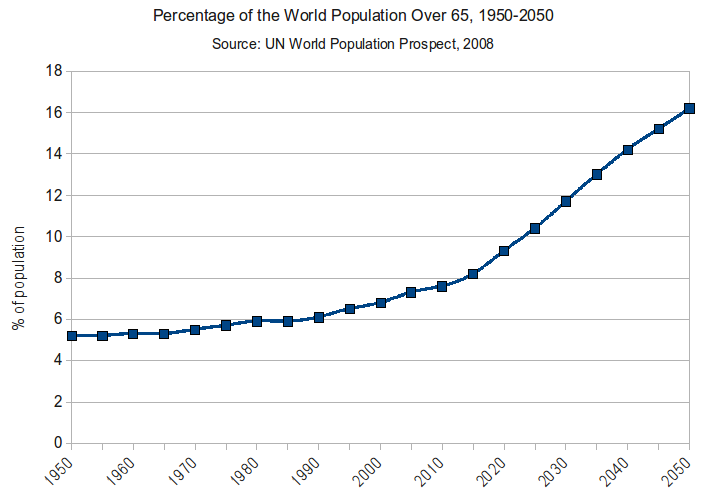
\includegraphics[scale=.5]{./gfx/populationOver65}
  \caption{Percentage of world population over 65, 1950--2050; \citep{populationAgeing}.\label{fig:agingPopulatiom}}
\end{figure}

% The Challenge
The problems of ageing population (see \emph{Figure~\ref{fig:agingPopulatiom}}), global population health issues, increasing healthcare costs, and decreasing quality of life are addressed by the \emph{SPHERE Project} hosted at the University of Bristol \citep{sphere}. This collaboration of clinicians, engineers, designers, social care professionals and various members of the public develops helpful technologies addressing real healthcare problems in a cost effective way.\\
The project focuses on developing real-world technologies which are acceptable in people's homes i.e.\ do not hindering everyday-life. SPHERE works on both hardware and software smart house solutions: sensors and wearable devices as well as algorithms for healthcare applications. The first, are fitted in the place of interest to monitor it and generate various kind of signals, while the latter, use acquired information to identify medical or well-being issues: predict falls, detect strokes, analyse eating behaviour, and detect periods of depression or anxiety.\\
This project extends algorithmic part of undertaken by SPHERE research by proposing novel data analysis framework.

      \subsubsection{Smart City}
Despite huge popularity in healthcare, spatio-temporal data feeds can also be found in variety of monitoring applications. One of them described by \citet{filipponi2010smart} is smart-city management. Automatic analysis---quick and robust---of traffic information, accident reports, etc.\ is of invaluable help in case of emergency.\\
Among many possible applications, produced analysis can result in timely police intervention or well planned route for emergency services, therefore, help in evacuation, crowd management, terrorist attack prevention and airport security control.

      \subsubsection{Complex Systems}
Spatio-temporal data is also produced in large quantities by many of complex systems monitoring and control devices, e.g.: scientific facilities, buildings, data centres~\citep{moore2005data} and power plants~\citep{amin2005toward}. 
Tasks impossible to handle by humans either due to large data volume throughput or demand for low response time are vast area of application for spatio-temporal data analysis. Such tools facilitate well suited for needs system management and risk detection. Power distribution and balancing, nuclear reactor control, data centre heat management are such tasks to name a few.

      \subsubsection{Wildlife}
Monitoring animals behaviour in their natural habitat is an important source of information for many researchers~\citep{Szewczyk:2004:HMS:990680.990704}. Nevertheless, this task is very often impractical either due to adverse climate or difficult access to monitored place. Moreover, scientists in many cases want to avoid disturbing animals' life-cycle and habitats. Difficult access to such sites can be easily overcome with wide range of available sensors and analytic tools, which share common ground with activity recognition model.


  \section{Contribution}
    \subsection{Existing work}
I don't know any existing work.

    \subsection{Project contribution}
The main aim of the project is to apply Inductive Logic Programming techniques to spatio-temporal data generated by smart installations like houses and cities, in order to build \emph{Activity Recognition Model}. Such model describes each monitored activity with a set of \emph{first-order logical rules} built with events, where each event is based on sensor readings. Example of ILP rules learnt with \texttt{Prolog} are shown in \emph{Listing~\ref{lst:eg}}.

What is my bit ->
No single classifeir can handle versatility of structer hidden in the data
Therfore for it to be most effective it needs to be ensemble of classifier where each covers area (strong points) not covered by any other
-> GENERAL SOLUTION
CRF are widely used due to their ...
they mainly use motion sensors
BUT they are data specific - learn model is not universal
its fairly 
-> MY SOLUTION
Prolog rules and ILP
rules can be farly easy read by a human
rules can be easly manipulated
rules can be extended by natural grama generation -> plain english
rule base dmodel can become -> a generative model for data
rules can be translated into new features -> Furthermore, such model can be used to build new features: in presented above example both \texttt{location} and \texttt{device} rules can be transformed to become features. Rebuilt dataset may become more ``informative'' than the original one, therefore, it can improve classification carried out with variety of different machine learning models.
rules are easy to expand -> different level of depth - meal -> type of meal -> based on used ingredients

\section{Techniques}
Techniques used -> why I think it's best for the problem -> more details
datasets from CASAS
Data generation
ILP
Prolog used
Cross validation

\section{Deliverables}
Deliverables / contribution -> what the project will result in
data generator that produces real like data
rules for activity (that are considered difficult to recognise) recognition of single person in house
rules for multiple residents in the house

\section{Challenges}
Lack of labelled data to train and test models -> not knowing what is in real data -> therefore neeed to emulate some to check it out
time represenataition - unbounded variable in aI and ILP: time and real-valued sensors
data noise and incompleteness
Information loss: room and sensor layout
incompleteness and noise in the data
tuning ILP systemin this case ALEPH, to build activity recognition model
design of features to extract relevant information form data
design of background knowledge to extract the features
prediction continuity issues, and readings in time continuity issues
adjusting resolution of the rules -> detail of prediction -> meal -> what kind of meal -> etc. -> level of depth -> dicover hierarchy -> chain of sub-activities contributing to the main action, or state which sensor or sequence of sensors build such actions.
what evaluation techniques to use -> multiple error possibilities
multiple residents dicovery -> Most often monitored places are inhabited or being used by multiple people. Another important task that can be performed with proposed technique is identifying actions and agents associated with them when multiple users simultaneously share observed space.

Very often the data collected from smart houses is corrupted or obscure due to sensor noise, leading to confusing gaps between ``observed'' actions. With help of inductive learning such implicit information---describing intermediate steps between actions---can be inferred to overcome rule creation difficulty and produce logically consistent scenario. This in turn can be translated into natural language using second ``grammar''.\\

Finally, data derived from smart houses is highly structured. Human activities can be hierarchically organised with complex actions composed of sub-actions, until ``atomic level'' is reached. This creates possibility to apply filters to produce multiple levels of narrative complexity based on target audience. Adjusting level of detail (granularity) of produced description would result in emphasis on different aspects of carried out activities during period of interest, hence, extracting relevant for the audience information.

\section{Result evaluation}
OUtput asses ->
assess the generator by applying models learnt on real data and on generated data to prove bidirectionality
use cross validation with random bits in generated data
use models learnd on data and vice versa to assess it
used CRF on both generated data and real data to compare results
genuine data can be split per person (each person doing 5 diff activities) -> cross validated
single occupier data can be coverteed to ARFF format and different models in Weka can be used to check it out



%===============================================================================
%===============================================================================
%===============================================================================
%===============================================================================
%===============================================================================
\chapter{Spatio-temporal data\label{ch:stData}}
Introduce the data
--CASAS example
--What the data looks like
--Problems with the data -> hard to learn activity models

The generator
--Capabilities
--Advantages
--Design activities and learn them
--Proof of the generator producing real-life data
--ILP ready:
----generates background knowledge, positives, negatives, and location activity details

The converter
--Convert CASAS-like data to knowledge representation
--Generate positive and negative examples
--Handles both single and multiple residents

Cross-validation
--Performs cross-validation on learnt rules and generated data
--Reports statistics per label (activity) and overall performance

Knowledge representation of spatiotemporal data
--Data example - 4 time representations
--Background knowledge makes learnt rules universal




\subsection{Unbounded sensor readings}
just treshold them\\
info about spatio temporal data --- why they are so important and wide spread\\

\section{Used datasets}
The spatio-temporal class of data is of interest. Data-points in such sets are characterised by both location and time of the event. Such data are generated by all smart instillations like houses and cities. In this study smart house data are used but the generalisation of the solution is straight forward.\\ % specification

The datasets used for model building and testing are ones generated at \emph{Washington State University} as part of \emph{CASAS} project~\citep{cook2009assessing}. \emph{WSU Smart Apartment ADL Normal Testbed} and \emph{WSU Smart Apartment ADL Error Testbed} are the two most popular ones hence are used in the project.\\

The datasets are structured as a list of sensor readings---one entry per line in format: \texttt{Date}---\texttt{Time}---\texttt{SensorID}---\texttt{Value}. The fragment of such dataset is presented in \emph{Listing~\ref{lst:data}}.

% \vspace{1em}
\begin{figure}
\lstset{
  captionpos=b,
  frame=single,
  language=HTML,
  breaklines=true,
  caption=CASAS dataset structure.,
  label=lst:data,
  float=tb
}
\begin{lstlisting}
...
2008-02-26 10:52:58.577436 M17   OFF
2008-02-26 10:52:59.648222 M18   OFF
2008-02-26 10:52:59.792264 M17   ON
...
2008-02-26 10:53:43.512642 I02   ABSENT
2008-02-26 10:53:43.978491 I01   ABSENT
...
2008-02-26 10:53:52.112690 AD1-B 0.0421491
2008-02-26 10:53:54.721822 M17   ON
2008-02-26 10:53:55.107910 AD1-B 0.155979
...
\end{lstlisting}
\end{figure}
% \vspace{1em}

The datasets were generated with sensors fitted into living space of house and agents performing predefined activities. The following sensors were used:
\begin{description}
\item[M\_\_] motion sensors.
\item[I\_\_] item sensors e.g.\ oatmeal, raisin, brown sugar, bowl, measuring spoon, medicine container, phone book.
\item[D01] cabinet sensor.
\item[AD1-A, AD1-B] water sensor.
\item[AD1-C] burner sensor.
\item[asterisk] phone usage.
\end{description}

The sensor layout of the apartment is shown in the \emph{Figure~\ref{fig:house}}.

\begin{figure}[htb]
  \centering%[width=.45\textwidth]
  \begin{subfigure}[b]{0.6\textwidth}
    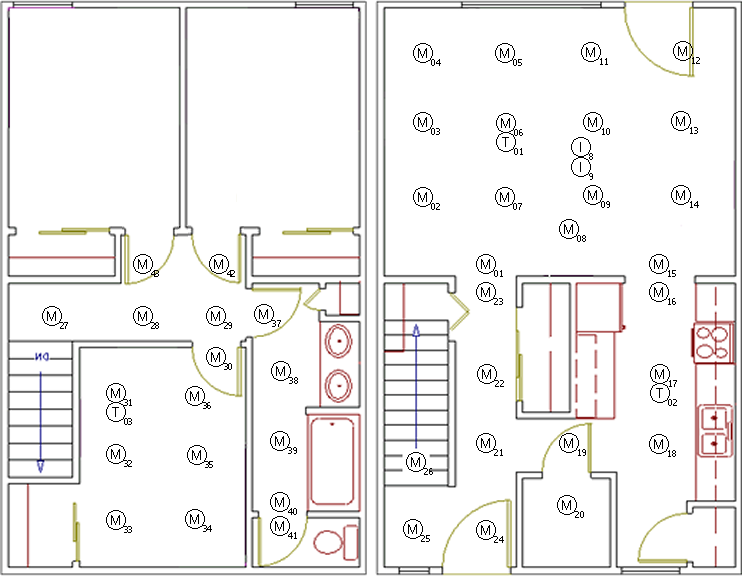
\includegraphics[height=6.3cm]{gfx/Chinook_3_Bedroom_TH}
    \caption{\label{fig:house:a}}
  \end{subfigure}%
  \begin{subfigure}[b]{0.3\textwidth}
    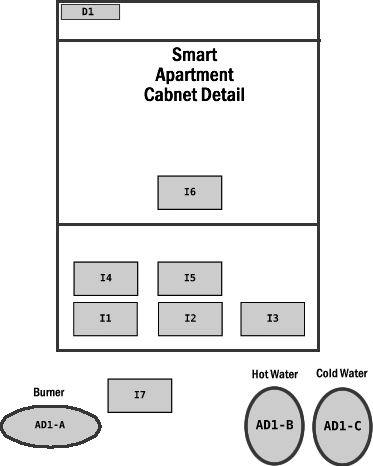
\includegraphics[height=6.3cm]{gfx/Chinook_Cabinet}
    \caption{\label{fig:house:b}}
  \end{subfigure}%
  \caption[The sensor layout of the apartment.]{The sensor layout of the apartment~\citep{cook2009assessing}.\label{fig:house}}
\end{figure}

Participants performed five \emph{Activity of Daily Living}(ADL) tasks:
\begin{description}
\item[Make a phone call] Move to the phone in the dining room; find a specific number in the phone book; dial the number; listens to the message; summarise cooking directions provided over the phone on a notepad.
\item[Wash hands] Move into the kitchen; wash hands in the sink with hand soap; dry hands with a paper towel.
\item[Cook] Cook a pot of oatmeal according to the directions given in the phone message: measure water, pour the water into a pot; boil the water; add oats; put the oatmeal into a bowl; add raisins and brown sugar.
\item[Eat] Take cooked oatmeal; take medicine container; move to the dining room; eat the food.
\item[Clean] Take all of the dishes to the sink in the kitchen; clean them with water and dish soap.
\end{description}


\section{Time representation}
4 different time representations
sequence is most suitable for this application
not sparse numbers hich are easy to iterate without exhaustive serch
but additionally timestamp is great source of information
as its of a magnitude $10^{16}$ (micro-seconds $\mu$-seconds)
but you can extract time differenc of any two sensor activations -- time elapsed since given event -- and treshold it
and finally and most notably you can discretise time stamps which is a lot easier than working with numbers in ilp and AI namely:
  time of year (winter, summer autumn, spring), month: jan, feb, , time of day: morning, afternoon, evening, night




\section{Data generator}

\begin{figure}
  \centering
  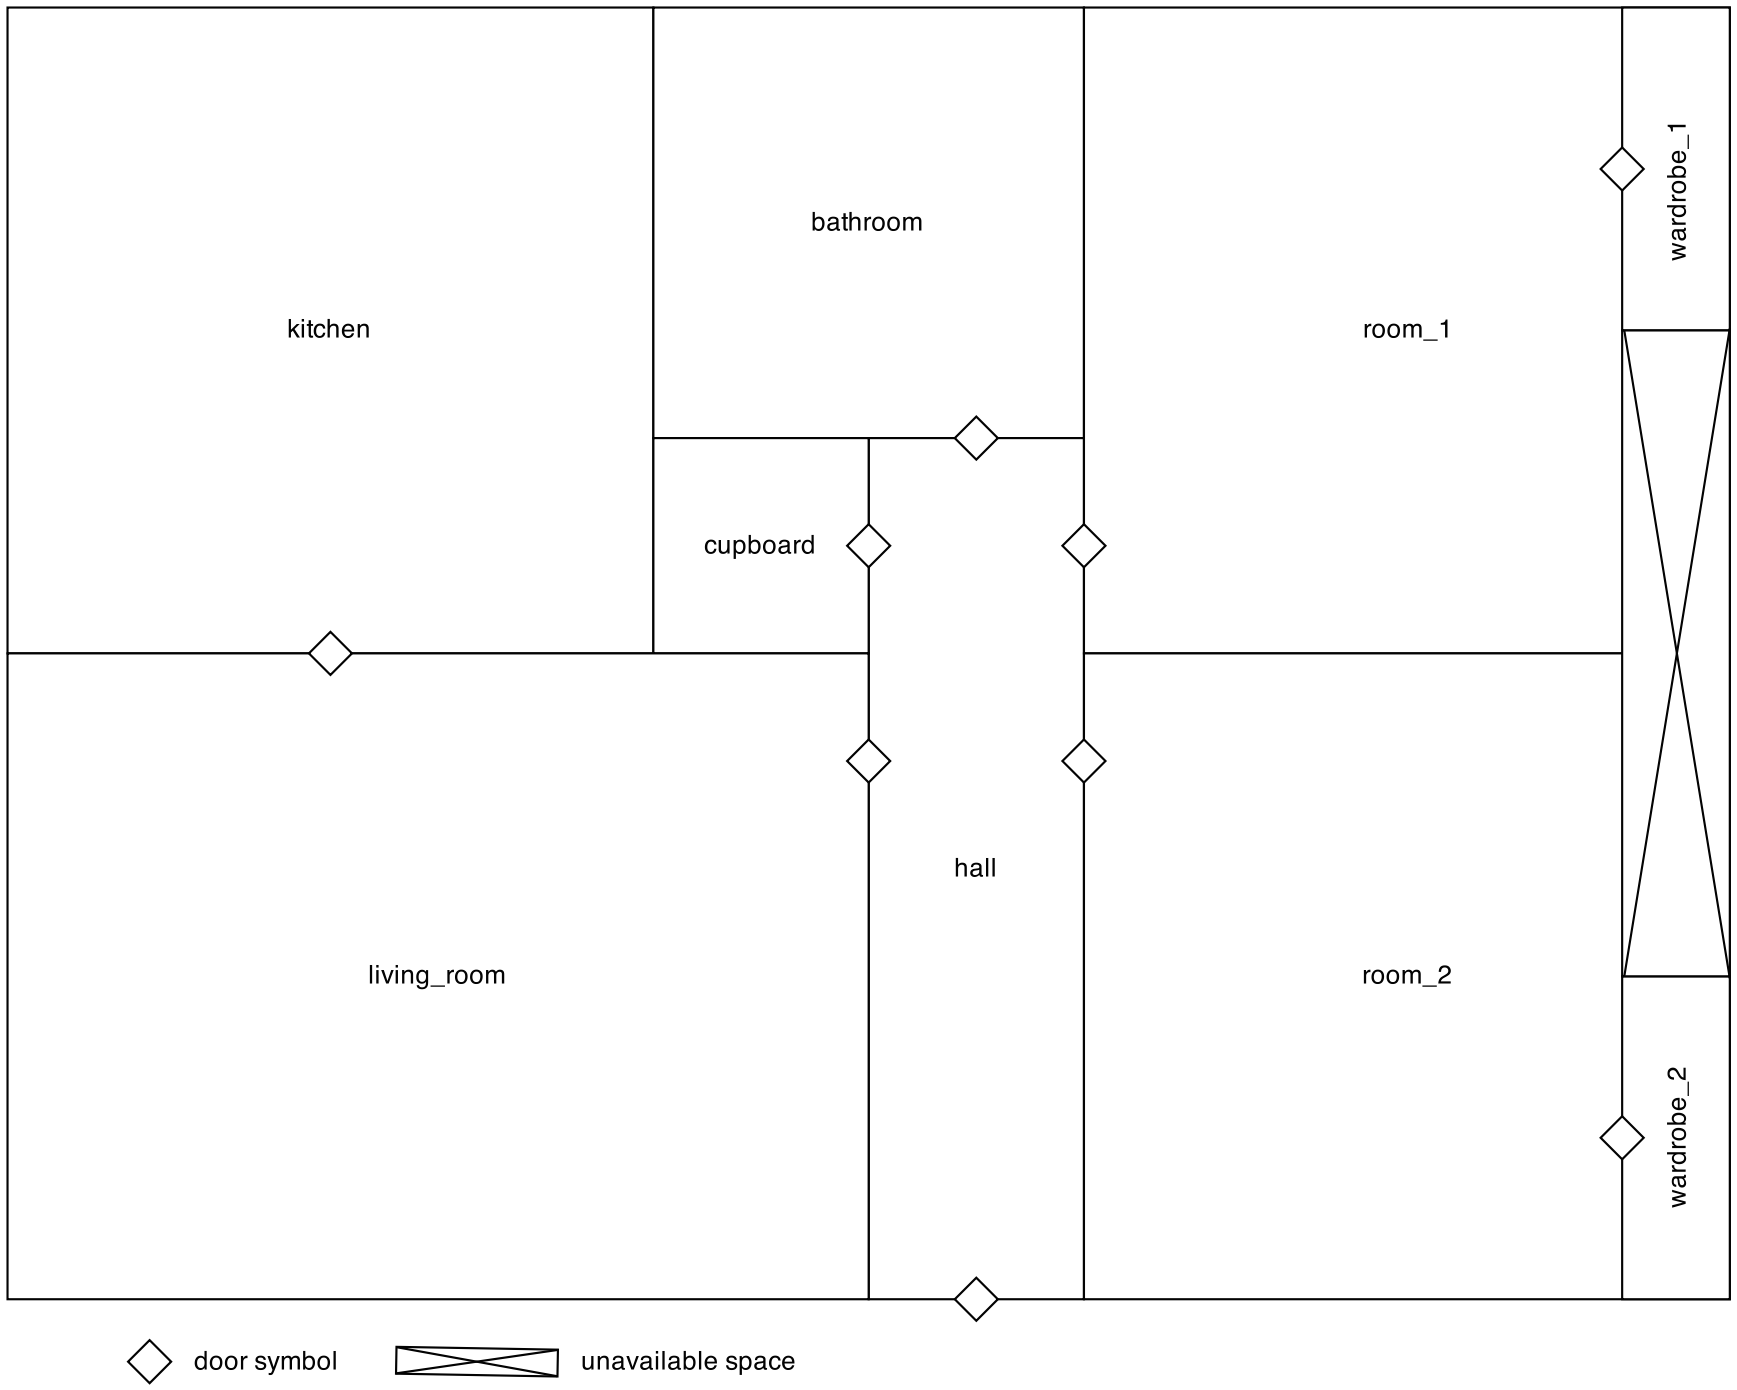
\includegraphics[width=.9\textwidth]{./gfx/room_layout}
  \caption{Room layout of simulated house.}
\end{figure}

use coded background knowledge to generate data: sample path and sensor firing\\
tool to generate such data would be of great importance in testing and model building\\

data generator generates smart house data based on 4 description files:
\section{\texttt{rooms.l}}
Defines interconnection of rooms in form of an adjacency matrix:\\
% \lstinputlisting[language=Python]{../stdg/rooms.l}

The first element in first line must be \texttt{[X]}\\
The headers must be \emph{roomName} --- must be without spaces.

\section{\texttt{activities.l}}
This file specifies the parameters of Gaussian distribution describing \emph{activities names} in form of:\\
\texttt{nameOfActivity mean standardDeviation}

it is used to simulate time needed to accomplish activity in \emph{seconds}.

% \lstinputlisting[language=Python]{../stdg/activities.l}

\section{\texttt{path.l}}
This files describe activities to generate in form \texttt{keyword(goal)}:\\
% \lstinputlisting[language=Python]{../stdg/path.l}

the \texttt{keywords} in this file are:\\
\begin{description}
\item[\texttt{start}] where the person starts
\item[\texttt{go}] where to go
\item[\texttt{do}] what activity to do
\end{description}

The \texttt{goals} are:
\begin{description}
\item[room names] defined in \texttt{rooms.l} file and matched with \texttt{go} or \texttt{start} keywords

\item[activities] have to be defined in both \texttt{activities.l} and \texttt{layout.l} files; are matched with \texttt{do} keywords
\end{description}


this file must start with command \texttt{start}\\
to \texttt{do} given activity you first must go to the room that it is available in.

\section{\texttt{layout.l}}
All measures are in meters\\
the room layout description is based on cartesian coordinates with origin in bottom left corner\\

This file defines sensor layouts for each of the rooms defined in \texttt{rooms.l} file:\\
% \lstinputlisting[language=Python]{../stdg/layout.l}

each room has to be described as:
\texttt{roomName} \texttt{widthOfRoom} \texttt{heightOfRoom} \texttt{:}\\
The room description line has to be finished with \texttt{:}, without spaces.\\

followed by sensors descriptions:\\
\texttt{motionSensorID} \texttt{widthOfSensorLocation} \texttt{heightOfSensorLocation} \texttt{rangeOfSensorRadius}\\
or
\texttt{itemSensorID} \texttt{widthOfSensorLocation} \texttt{heightOfSensorLocation} \texttt{activityName}\\
or\\
door description starting with \texttt{door} keyword and finished with \texttt{roomName} to which the door lead:\\
\texttt{door} \texttt{widthOfSensorLocation} \texttt{heightOfSensorLocation} \texttt{roomName}\\

comment lines start with \texttt{;}\\


\section{\texttt{aleph.pdf}}
The basic algorithm(page 4):\\
\begin{enumerate}
  \item Select example.
  \item Build most-specific-clause.
  \item Search.
  \item Remove redundant.
\end{enumerate}

Needed files:
\begin{enumerate}
  \item Background
  \item Positives
  \item Negatives
\end{enumerate}





%===============================================================================
%===============================================================================
%===============================================================================
%===============================================================================
%===============================================================================
\chapter{Inductive Logic Programming\label{ch:ILP}}
\section{Main concept}

\begin{figure}
  \centering
  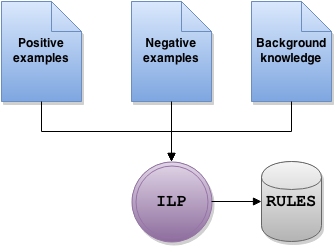
\includegraphics[scale=.5]{./gfx/ilp}
  \caption{ILP scheme\label{fig:ilp}}
\end{figure}

\section{\texttt{ALEPH}}
\section{Applications to spatio-temporal data}
pros and cons Use of background knowledge
\section{Least general generalisation}
activity description
\section{Feature discovery and feature extraction}

-----

\citeauthor{plotkin1972automatic} in early 1970s and \citeauthor{shapiro1983algorithmic} in early 1980s created foundation of \emph{Inductive Logic Programming}(ILP). Both authors introduced techniques and tools to learn \emph{first-order formulas}---parametrised rules that are the core of ILP---from set of facts. Since then, ILP techniques found number of interdisciplinary applications with new tools being created now and then for rules learning purposes.

\section{Inductive Logic Programming}
The concept of Inductive Logic Programming is based on fusion of two well known techniques: \emph{inductive learning} and \emph{logic programming}. The first component facilitates building model from available observations and generating new knowledge form experience. The latter, introduces a powerful representation of knowledge as \emph{first-order logical rules}~\citep{muggleton1994inductive,muggleton1995inverse}.\\

First-order logic is more powerful than widely used \emph{propositional logic}, which builds sentences (i.e.\ rules) with facts only by using logical connectives. The first, extends propositional logic by using as part of the rules quantified variables (i.e.\ parameters) that belong to some domain of interest. The major limitation of first-order logic is its restriction to finite variable domains---it cannot describe rules built on infinite sets like real or natural numbers.\\ %  as opposed to

The power of ILP is inherited from first-order logical rules that it is built upon. First of all, ILP overcomes the use of ``limited representation formalism''---expressing data in form of a propositional logic. As many problems cannot be expressed propositionally, but it is possible in some form of first-order logic, previously difficult to solve problems can be easily tackled.\\
Moreover, ILP does not have difficulties in incorporating substantial background knowledge to the model in learning process. This feature is not very common among machine learning models, nevertheless, use of domain knowledge is ``essential for intelligent behaviour''~\citep{muggleton1994inductive}.\\

Constructing \emph{first-order clausal theories} i.e.\ hypotheses is based on combining background knowledge with information represented as facts: positive and negative examples. ILP aims at building theory that explains facts under consideration of background knowledge.\\
To this end, it uses \emph{induction} as a basic mode of inference---generalization of specific observations to theories, rather than deduction---transforming general theories to the more specific clauses.\\

The rules produced with ILP are human readable unlike models produced by majority of machine learning solutions, what gives it great advantage over competition. Easy to understand rules means that the logic models are arguably easy to manipulate. They can be changed by simply adding, deleting, and appending clauses or literals.\\

Such model representation is invaluable in \emph{scientific theory formation} and problems where data cannot be easily represented in attribute-vale language. ILP is widely used in structure-activity prediction for drug design~\citep{king1992drug,michael1992modelling} and protein secondary-structure prediction~\citep{muggleton1992protein}.\\
It is also popular in computer science in: programming assistants, algorithmic debugging, program testing and verification, and reverse engineering~\citep{shapiro1983algorithmic,bergadno1993inductive,bratko1993inductive}.\\

To construct Activity Recognition Model two popular ILP \texttt{Prolog} implementations are examined: \texttt{Aleph}\footnote{\url{http://www.cs.ox.ac.uk/activities/machlearn/Aleph/aleph.html}} and \texttt{Progol}\footnote{\url{http://www.doc.ic.ac.uk/~shm/progol.html}}.



\section{Background knowledge}
not possible to give experiment design and structure in data\\
possible to recover partialy but hard to do, time consuming\\

in prolog and ILP it an be represent and used as knowledge:\\
structure of rooms\\
ensor layout\\


\section{Closed Concept \& Least General Generalisation}
keep not needed clauses in body.

``A closed concept is a concept where all the necessary and sufficient conditions required to include something within the concept can be listed. For example, the concept of a triangle is closed because a three-sided polygon, and only a three-sided polygon, is a triangle. All the conditions required to call something a triangle can be, and are, listed.''



%===============================================================================
%===============================================================================
%===============================================================================
%===============================================================================
%===============================================================================
\chapter{Sequential multi-class model---single resident\label{ch:smcm}}
Simple generated datasets\\
Synthetic CASAS \#2 -- narrated datasets\\
CASAS \#2 -- narrated datasets\\
Continuity rule -- introducing bias\\
Meta-rule -- smoothing out predictions\\
Generality of learnt rules (synthetic <--> genuine) Results overview\\
Overlapping activities -- single resident multi-label case\\


\vspace{1em}
\begin{figure}[htb]
\lstset{
  captionpos=b,
  frame=single,
  language=Prolog,
  breaklines=true,
  caption=Example of target rules.,
  label=lst:eg,
  float=tb
}
\begin{lstlisting}
activity(Person, cooking) :- location(Person, TimeWindow, kitchen), device(TimeWindow, hob).
activity(Person, watchingTV) :- location(Person, TimeWindow, livingRoom), device(TimeWindow, tv).

location(Person, TimeWindow, kitchen) :- sensor(1, on, TimeWindow), sensor(5, on, TimeWindow).
location(Person, TimeWindow, livingRoom) :- sensor(2, on, TimeWindow), sensor(7, on, TimeWindow).

device(TimeWindow, hob) :- sensor(101, on, TimeWindow).
device(TimeWindow, tv) :- sensor(105, on, TimeWindow).
\end{lstlisting}
\end{figure}





%===============================================================================
%===============================================================================
%===============================================================================
%===============================================================================
%===============================================================================
\chapter{Multi-label model---multiple residents\label{ch:mlm}}


%===============================================================================
%===============================================================================
%===============================================================================
%===============================================================================
%===============================================================================
\chapter{Summary\label{ch:summary}}
Data generator as a helpful tool for building and testing models\\
ILP can be used as one of models for activity recognition: its strong points not available (or hard to achieve) in other models
Further development: data narration

---

\section{Further development: Data Narrative\label{sec:narrative}}

Proposed here ILP tool could extend suit of available analytic technologies for activity recognition and become great foundation for \emph{Narrative Analtics} presented in \emph{Section~\ref{sec:narrative}}.

Proposed here rules learning mechanism can be extended with ``grammar'' capable of generating \emph{Narrative Analysis} of spatio-temporal data: a \emph{succinct natural language description} of a selected time-space window of the data of interest. In healthcare and smart house scenarios, such techniques can be combined with activity recognition models to generate comprehensible descriptions of monitored activities with terminology and level of detail tuned to a particular recipient. In the context of the SPHERE project these techniques would facilitate making sense from acquired data for healthcare applications in a more transparent way than is possible with black-box approaches.

  \subsection{Visualisation techniques}
Most commonly used visualisation techniques nowadays are tables, graphs, and diagrams. Unfortunately, such charts often need expertise in a field to be correctly interpreted. Moreover, aforementioned methods often trade-off clarity for completeness of shown data hence make it difficult for a broad audience to see the big picture.\\

\emph{Narrative Analysis} aims at exploring possibility of describing data with natural language. This form of expressing information contained in the data has been under-appreciated and devoted little attention in recent years. Deep learning techniques have been applied to images to generate succinct scene description, nevertheless, it has not been used with raw data.\\
An example of data narration can be found in modern smart-phone weather and calendar applications where instead of detailed weather forecast or hour-by-hour calendar events, one sentence description is presented to the user. Furthermore, in recent years \emph{narrative analytics} in combination with visualisation techniques have been proven as effective method of expressing corporate financial data.\\

Successful adaptation of \emph{Narrative Analytics} to data provided by smart houses would greatly benefit healthcare applications. Being able to deliver activity description within given time-space window and with different level of detail would provide invaluable monitoring and diagnostic tool for daily care personnel and medical staff.

  \subsection{Narrative Analytics}
Presented here extension is not restricted to smart house data. \emph{Narrative Analytics} can be applied to any spatio-temporal information---e.g.\ smart-city feed---resulting in brief situation description contained in the data. Such ``label'' gives possibility to quickly understand status of the system without time-consuming raw-data or charts interpretation. Improved response time would result in appropriate actions taken instantly, whether it is better disease diagnosis, or traffic conditions displayed in timely manner on interactive information signs.\\
Moreover, as produced description would also be hierarchical it can be formed in a ``tree'' structure with more general narratives being higher in hierarchy. Creating timetable filled with activity ``labels'' would give better insight into personal habits and routines yielding improved understanding of arising issues.\\
Furthermore, proposed here descriptive mechanisms could be extended to become a query-enabled database. In such model a user could ``ask'' a question in natural language to get narrative answer instead of numerical vector.\\

Data narration can have multiple other applications. Alternatively, it can be used to produce figure caption based on data used to draw it.

  \subsection{Challenges}
Creating a narrative of events is composed of two major components---``grammars'' needed to transform the data: \emph{data analysis}(objective of this project) and \emph{narrative generation}.\\
The first one is deriving high-level knowledge from low-level data (sensor input) with ILP. The latter is ``translating'' extracted information into natural language description, which also can be done using similar approach.


\begin{center}
\noindent \line(1,0){250}
\end{center}

\bibliography{yhpargoil}{}
\bibliographystyle{plainnat}
% \bibliographystyle{plain}

\end{document}

% useful expressions:
%% aggregate signal
